%%%%%%%%%%%%%%%%%%%%%%%%%%%%%%%%%%
%%%%%%%%%%%%%%%%%%%%%%%%%%%%%%%%%%
%Plantilla pel Treball Fi de Grau
%%%%%%%%%%%%%%%%%%%%%%%%%%%%%%%%%%
%%%%%%%%%%%%%%%%%%%%%%%%%%%%%%%%%%%%%%%%%%%
\documentclass[twocolumn]{revtex4}
%%%%%%%%%%%%%%%%%%%%%%%%%%%%%%%%%%%%%%%%%%%
\usepackage{graphicx,epsfig}
\usepackage{amsmath}
\usepackage{amsfonts}
\usepackage{fancyhdr}


\newcommand{\keyword}[1]{\noindent{\bf Keywords: }{#1}\\}
\newcommand{\keywordcat}[1]{\noindent{\bf Paraules clau: }{#1}\\}
\newcommand{\sdg}[1]{\noindent{\bf SDGs: }{#1}\\}
\newcommand{\ods}[1]{\noindent{\bf ODSs: }{#1}\\}

%%%%%%%%%%%%%%%%%%%%%%%%%%%%%%%%%%%%%%%%%%%
%%%%%%%%%%%%%%%%%%%%%%%%%%%%%%%%%%%%%%%%%%%
\makeatletter
\def\maketitle{
\@author@finish
\title@column\titleblock@produce
\suppressfloats[t]}
\makeatother
%%%%%%%%%%%%%%%%%%%%%%%%%%%%%%%%%%%%%%%%%%%

\begin{document}



%%%%%%%%%%%%%%%%%%%%%%%%%%%%%%%%%%%%%%
\pagestyle{fancy}
\lhead{\bf TITLE}
\rhead{Student's name}
\lfoot{Treball de Fi de Grau}
\rfoot{Barcelona, \today}
%%%%%%%%%%%%%%%%%%%%%%%%%%%%%%%%%%%%%%


\title{Precise computation of AOD holograms via AI modelling}
\author{Author: Guillermo Ramos Ramiro, gramosra7@ub.edu}
\affiliation{Facultat de F\'{\i}sica, Universitat de Barcelona, Diagonal
645, 08028 Barcelona, Spain.}
\author{Advisor: Mario Montes Usategui, mario_montes@ub.edu}

\begin{abstract}
{\bf Abstract:} Some examples of the use of \LaTeX , for styles, sections, figures, tables, formulas, references, and other details are provided here with specific information and guidelines that should be read carefully before starting to write the manuscript for the Treball Fi de Grau (TFG). Note that the report must be written in English, but on the sixth page, the title, summary, and keywords in Catalan must be included. The sixth page should also contain a brief comment relating the TFG to the Sustainable Development Goals (SDG). The abstract should concisely cover the objectives, methods and data used, results, and conclusion, and it should be 100 to 150 words in length.

\keyword{Up to 6 key words to correlate your work with the Physics degree's subjects}
\sdg{Enumerate the sustainable-development goals (ODS) this work is related to (see page 6)}
\end{abstract}


\maketitle

%%%%%%%%%%%%%%%%%%%%%%%%%%%%%%%%%%%%%%%%%%%%%%%%%%%%%%%%%%%%%%%%%%%%%%%%%%%


\section{Introduction}
In this document you will find the structure as well as the length
of what the {\it Treball Fi de Grau} (TFG) report is
required to have. It uses
\LaTeX\ in a two-column format and provides an example of what the essay
ought to look like, including lists, tables and figures.

The text has to be written in (good) English (compulsory).
The length of the report should by no means exceed {\bf five} pages in the
present format,
all figures, tables, etc..., included. It is important that the
two requirements are precisely met. Otherwise the essay will not be
considered for evaluation, and will automatically fail with
a mark of {\it Susp\`es}.

The report must consist of the following parts:
\begin{enumerate}
\item Abstract
\item Introduction
\item Development sections
\item Conclusions
\item Bibliography
\item Appendix (Optional)
\end{enumerate}


The final score will combine both the
advisor and the jury marks.
The defense will consist of a 15 minute public presentation before
a jury composed by two members. The deadlines as well as the dates for the
presentations will be announced in due time.
The students are encouraged to stick to the allowed allotted time (15 minutes),
since no extra time will, in general, be conceded by the jury members.
At any rate,
it should be clear that a list of conclusions needs to be read
before the presentation is over.

The evaluation will follow the {\it R\'ubriques} (or {\it Taules
d'avaluaci\'o}) provided by the TFG Advisory Committee,
which will be available to
the students prior to the presentation date, well ahead of time. It is
highly advisable for the students to read them thorough and carefully,
in order to become aware of all the competences that need be assessed
to comply with the guidelines of Bologna.

Make sure that the presentation will include:
\begin{enumerate}
\item Introduction.
\item Development sections.
\item Conclusions.
\end{enumerate}

You can find all the information concerning the TFG process in,
\begin{verbatim}
https://www.ub.edu/portal/web/fisica/tramit-tfg
\end{verbatim}

%%%%%%%%%%%%%%%%%%%%%%%%%%%%%%%%%%%%%%%%%%%%%%%%%%%%%%%%%%%%%%%%%%%%%%%%%
\section{Equations: a few examples}
Let us write a few equations,
\begin{equation}
\Delta =\sum_{i=1}^N w_i (x_i - \bar{x})^2,
\label{eq:1}
\end{equation}
with a label so that we can refer to it later. For instance you can refer
to it as Eq. (\ref{eq:1}).
All equations must be numbered.
If needed, you can also produce unnumbered equations.
\begin{equation}
T = 2 \pi \sqrt{\frac{l}{g}}. \nonumber
\end{equation}
You can insert equations in the text, like $e^{i \pi} +1=0$;
$\frac{df(x)}{dx}$ or you may prefer
$\displaystyle \frac{df(x)}{dx}$.
You can also write aligned equations,
\begin{eqnarray}
\frac{du(x)}{dx}+V u(x) +W v(x) &=& (\lambda + \alpha)  \; u(x) \nonumber \\
\frac{dv(x)}{dx}+V v(x) +W u(x) &=& (\lambda - \alpha) \; v(x).
\label{eq:tercera}\end{eqnarray}
Further examples are,
\begin{eqnarray}
\nabla {\cdot} \vec{E}&=& 4 \pi \rho \nonumber \\
\nabla \times \vec{B} - \frac{1}{c} \frac{\partial \vec{E}}{\partial t} &=&
\frac{4 \pi}{c} \vec{J} \nonumber \\
\nabla \times \vec{E} +\frac{1}{c} \frac{\partial \vec{B}}{\partial t} &=&
0 \nonumber \\
\nabla {\cdot} \vec{E}&=& 0,
\label{maxwell}
\end{eqnarray}
as can be found in \cite{jackson}, pag. 14. Also,
\begin{equation}
E = -J \sum_{i=1}^N s_i s_{i+1}.
\label{eq:ising}
\end{equation}

You can define your own macros to save typing
\footnote{This is a footnote.}.
For example, suppose
that you introduce a macro as follows:
\newcommand{\El}{{\vec{E}(\vec{x},t)}}
\begin{verbatim}
\newcommand{\El}{{\vec{E}(\vec{x},t)}}
\end{verbatim}
Then, by simply typing,
\begin{verbatim}
$\El$
\end{verbatim}
you get the electric field $\El$ printed out (in math mode, of course).

\vspace*{0.5cm}
You can write $\tilde x$,
$\overline{A}$; \%, accents: Schr\"odinger
and \'e, \`a, \`A, Mart\'{\i}; cal\c cotada,
$A \equiv B $, $\vec{A}\cdot\vec{B}$, $\vec{A} \times \vec{B}$,
$\vec{v}$, $\hat{n}$,
$c \sim d$, $z \approx w$, $\langle x \rangle$,
$\langle \psi | X | \psi \rangle$, $\hbar$, $g_{ij}$, $\delta^i_j$,
$R_{\mu \nu \alpha \beta ; \xi}$.

\vspace*{0.5cm}
You can also quote references easily, i.e., \cite{wmap}, \cite{weinberg}.

\vspace*{0.5cm}
A matrix
\begin{equation}
\left(
\begin{array}{ccc}
0 & 1 & 0 \\
1 & 0 & 1 \\
0 & 1 & 0
\end{array}
\right),
\label{matrix1}
\end{equation}
a vector (column)
\begin{equation}
\left(
\begin{array}{c}
1 \\
\sqrt{3}\\
\pi
\end{array}
\right),
\label{hola}
\end{equation}
a row,
\begin{equation}
\left(
\begin{array}{ccc}
p & q & r
\end{array}
\right),
\label{eq:row}
\end{equation}
and a determinant,
\begin{equation}
\left|
\begin{array}{ccc}
a_{11} & a_{12} & a_{13} \\
a_{21} & a_{22} & a_{23} \\
a_{31} & a_{32} & a_{33}
\end{array}
\right|.
\label{determinant}
\end{equation}

\noindent
Further examples:
\begin{equation}
\int_{-\infty}^\infty e^{-x^2} \, dx= \sqrt{\pi},
\label{eq:fine}
\end{equation}
also,
\begin{equation}
\int_a^b f'(x) \; dx=f(b)-f(a),
\label{barrow}
\end{equation}
and so on.

\subsection{Tables and figures}

An example of a table is shown in Table~\ref{tab:sample1}.

\begin{table}[h!]
\centering
\caption{Force, area, and pressure data for an experiment with glass syringes.}
\label{tab:sample1}
\vspace*{2mm}
\begin{tabular}{|l|l|l|}
\hline
& Piston 1 & Piston 2 \\
\hline
Force\,(N) & 4.40 & 2.25 \\
Area\,(cm$^2$) & 6.16 & 3.14 \\
Pressure\,(N/cm$^2$) & $0.714 \pm 0.002$ & 0.716 \\
\hline
\end{tabular}
\end{table}

Here we try to insert an illustrating figure, Fig.~\ref{fig:sample}.
For that you need to have created the figure before, in this case
the fig1.pdf file.

\begin{figure}[h!]
\centering
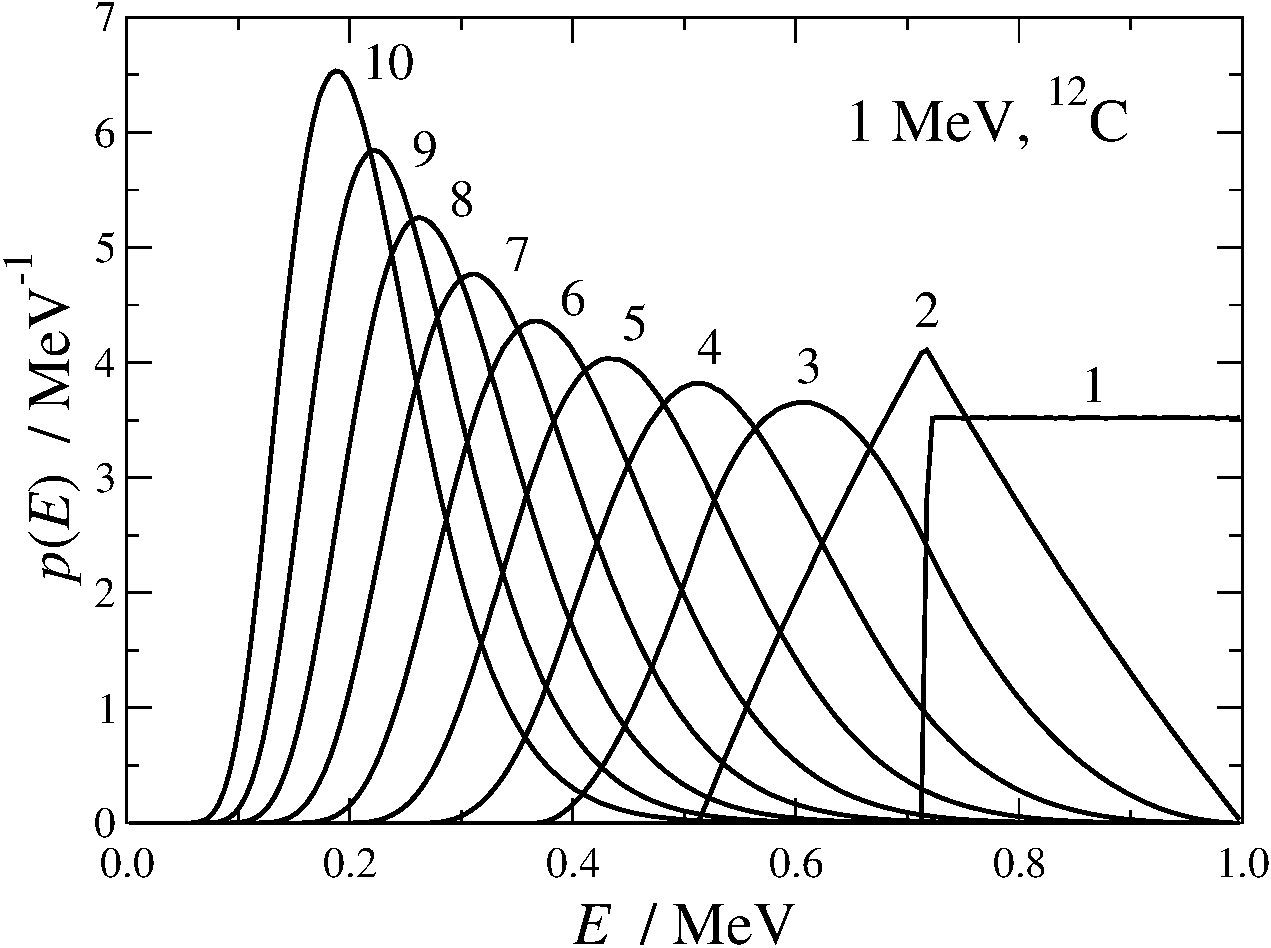
\includegraphics[width=\columnwidth]{fig1.pdf}
\caption{A sample figure.}
\label{fig:sample}
\end{figure}

%%%%%%%%%%%%%%%%%%%%%%%%%%%%%%%%%%%%%%%%%%%%%%%%%%%%%%%%%%%%%%%%%%%%%%%%
\section{Developing sections}
. . . . . . . . . . . . . . . . . . . . . . . . . . . . . . . . . . . . . . . .
. . . . . . . . . . . . . . . . . . . . . . . . . . . . . . . . . . . . . . . .
. . . . . . . . . . . . . . . . . . . . . . . . . . . . . . . . . . . . . . . .
. . . . . . . . . . . . . . . . . . . . . . . . . . . . . . . . . . . . . . . .
. . . . . . . . . . . . . . . . . . . . . . . . . . . . . . . . . . . . . . . .
. . . . . . . . . . . . . . . . . . . . . . . . . . . . . . . . . . . . . . . .
. . . . . . . . . . . . . . . . . . . . . . . . . . . . . . . . . . . . . . . .
. . . . . . . . . . . . . . . . . . . . . . . . . . . . . . . . . . . . . . . .
. . . . . . . . . . . . . . . . . . . . . . . . . . . . . . . . . . . . . . . .
. . . . . . . . . . . . . . . . . . . . . . . . . . . . . . . . . . . . . . . .
. . . . . . . . . . . . . . . . . . . . . . . . . . . . . . . . . . . . . . . .
. . . . . . . . . . . . . . . . . . . . . . . . . . . . . . . . . . . . . . . .
. . . . . . . . . . . . . . . . . . . . . . . . . . . . . . . . . . . . . . . .
. . . . . . . . . . . . . . . . . . . . . . . . . . . . . . . . . . . . . . . .
. . . . . . . . . . . . . . . . . . . . . . . . . . . . . . . . . . . . . . . .
. . . . . . . . . . . . . . . . . . . . . . . . . . . . . . . . . . . . . . . .
. . . . . . . . . . . . . . . . . . . . . . . . . . . . . . . . . . . . . . . .
. . . . . . . . . . . . . . . . . . . . . . . . . . . . . . . . . . . . . . . .
. . . . . . . . . . . . . . . . . . . . . . . . . . . . . . . . . . . . . . . .
. . . . . . . . . . . . . . . . . . . . . . . . . . . . . . . . . . . . . . . .
. . . . . . . . . . . . . . . . . . . . . . . . . . . . . . . . . . . . . . . .
. . . . . . . . . . . . . . . . . . . . . . . . . . . . . . . . . . . . . . . .
. . . . . . . . . . . . . . . . . . . . . . . . . . . . . . . . . . . . . . . .
. . . . . . . . . . . . . . . . . . . . . . . . . . . . . . . . . . . . . . . .
. . . . . . . . . . . . . . . . . . . . . . . . . . . . . . . . . . . . . . . .
. . . . . . . . . . . . . . . . . . . . . . . . . . . . . . . . . . . . . . . .
. . . . . . . . . . . . . . . . . . . . . . . . . . . . . . . . . . . . . . . .
. . . . . . . . . . . . . . . . . . . . . . . . . . . . . . . . . . . . . . . .
. . . . . . . . . . . . . . . . . . . . . . . . . . . . . . . . . . . . . . . .
. . . . . . . . . . . . . . . . . . . . . . . . . . . . . . . . . . . . . . . .
. . . . . . . . . . . . . . . . . . . . . . . . . . . . . . . . . . . . . . . .
. . . . . . . . . . . . . . . . . . . . . . . . . . . . . . . . . . . . . . . .
. . . . . . . . . . . . . . . . . . . . . . . . . . . . . . . . . . . . . . . .
. . . . . . . . . . . . . . . . . . . . . . . . . . . . . . . . . . . . . . . .
. . . . . . . . . . . . . . . . . . . . . . . . . . . . . . . . . . . . . . . .
. . . . . . . . . . . . . . . . . . . . . . . . . . . . . . . . . . . . . . . .
. . . . . . . . . . . . . . . . . . . . . . . . . . . . . . . . . . . . . . . .
. . . . . . . . . . . . . . . . . . . . . . . . . . . . . . . . . . . . . . . .
. . . . . . . . . . . . . . . . . . . . . . . . . . . . . . . . . . . . . . . .

\begin{table}[h!]
\centering
\caption{Another table.}
\label{tab:sample2}
\vspace*{2mm}
\begin{tabular}{||c||l|l|l||} \hline \hline
{\bf M1}  & Teoria:      & Galileo         & A11G \\ \cline{2-4}
 (11:45)  & Problemes:   & Newton          & A11G \\ \cline{1-4}
          & Problemes    & Planck (M1A)    & A11G \\ \cline{3-4}
 (12:45)  & tutoritzats: & Fermi (M1B)     & A23M \\
\hline \hline
{\bf M2}  & Teoria:      & Clausius        & A12G \\ \cline{2-4}
 (8:30)   & Problemes:   & Goeppert Mayer  & A12G \\ \cline{1-4}
          & Problemes    & Boltzmann (M2A) & A12G \\ \cline{3-4}
 (9:30)   & tutoritzats: & Maxwell (M2B)   & A24M \\
\hline \hline
{\bf T1}  & Teoria:      & Gibbs           & A12G \\ \cline{2-4}
 (18:00)  & Problemes:   & Helmholtz       & A12G \\ \cline{1-4}
          & Problemes    & Bohr (T1A)      & A12G \\ \cline{3-4}
 (19:00)  & tutoritzats: & Einstein (T1B)  & A24M \\
\hline \hline
\end{tabular}
\end{table}

\vspace*{0.5cm}

. . . . . . . . . . . . . . . . . . . . . . . . . . . . . . . . . . . . . . . .
. . . . . . . . . . . . . . . . . . . . . . . . . . . . . . . . . . . . . . . .
. . . . . . . . . . . . . . . . . . . . . . . . . . . . . . . . . . . . . . . .
. . . . . . . . . . . . . . . . . . . . . . . . . . . . . . . . . . . . . . . .
. . . . . . . . . . . . . . . . . . . . . . . . . . . . . . . . . . . . . . . .
. . . . . . . . . . . . . . . . . . . . . . . . . . . . . . . . . . . . . . . .
. . . . . . . . . . . . . . . . . . . . . . . . . . . . . . . . . . . . . . . .
. . . . . . . . . . . . . . . . . . . . . . . . . . . . . . . . . . . . . . . .
. . . . . . . . . . . . . . . . . . . . . . . . . . . . . . . . . . . . . . . .
. . . . . . . . . . . . . . . . . . . . . . . . . . . . . . . . . . . . . . . .
. . . . . . . . . . . . . . . . . . . . . . . . . . . . . . . . . . . . . . . .
. . . . . . . . . . . . . . . . . . . . . . . . . . . . . . . . . . . . . . . .
. . . . . . . . . . . . . . . . . . . . . . . . . . . . . . . . . . . . . . . .
. . . . . . . . . . . . . . . . . . . . . . . . . . . . . . . . . . . . . . . .
. . . . . . . . . . . . . . . . . . . . . . . . . . . . . . . . . . . . . . . .
. . . . . . . . . . . . . . . . . . . . . . . . . . . . . . . . . . . . . . . .
. . . . . . . . . . . . . . . . . . . . . . . . . . . . . . . . . . . . . . . .
. . . . . . . . . . . . . . . . . . . . . . . . . . . . . . . . . . . . . . . .
. . . . . . . . . . . . . . . . . . . . . . . . . . . . . . . . . . . . . . . .
. . . . . . . . . . . . . . . . . . . . . . . . . . . . . . . . . . . . . . . .
. . . . . . . . . . . . . . . . . . . . . . . . . . . . . . . . . . . . . . . .
. . . . . . . . . . . . . . . . . . . . . . . . . . . . . . . . . . . . . . . .
. . . . . . . . . . . . . . . . . . . . . . . . . . . . . . . . . . . . . . . .
. . . . . . . . . . . . . . . . . . . . . . . . . . . . . . . . . . . . . . . .
. . . . . . . . . . . . . . . . . . . . . . . . . . . . . . . . . . . . . . . .
. . . . . . . . . . . . . . . . . . . . . . . . . . . . . . . . . . . . . . . .
. . . . . . . . . . . . . . . . . . . . . . . . . . . . . . . . . . . . . . . .
. . . . . . . . . . . . . . . . . . . . . . . . . . . . . . . . . . . . . . . .
. . . . . . . . . . . . . . . . . . . . . . . . . . . . . . . . . . . . . . . .
. . . . . . . . . . . . . . . . . . . . . . . . . . . . . . . . . . . . . . . .
. . . . . . . . . . . . . . . . . . . . . . . . . . . . . . . . . . . . . . . .
. . . . . . . . . . . . . . . . . . . . . . . . . . . . . . . . . . . . . . . .
. . . . . . . . . . . . . . . . . . . . . . . . . . . . . . . . . . . . . . . .
. . . . . . . . . . . . . . . . . . . . . . . . . . . . . . . . . . . . . . . .
. . . . . . . . . . . . . . . . . . . . . . . . . . . . . . . . . . . . . . . .
. . . . . . . . . . . . . . . . . . . . . . . . . . . . . . . . . . . . . . . .
. . . . . . . . . . . . . . . . . . . . . . . . . . . . . . . . . . . . . . . .
. . . . . . . . . . . . . . . . . . . . . . . . . . . . . . . . . . . . . . . .
. . . . . . . . . . . . . . . . . . . . . . . . . . . . . . . . . . . . . . . .
. . . . . . . . . . . . . . . . . . . . . . . . . . . . . . . . . . . . . . . .
. . . . . . . . . . . . . . . . . . . . . . . . . . . . . . . . . . . . . . . .
. . . . . . . . . . . . . . . . . . . . . . . . . . . . . . . . . . . . . . . .
. . . . . . . . . . . . . . . . . . . . . . . . . . . . . . . . . . . . . . . .
. . . . . . . . . . . . . . . . . . . . . . . . . . . . . . . . . . . . . . . .
. . . . . . . . . . . . . . . . . . . . . . . . . . . . . . . . . . . . . . . .
. . . . . . . . . . . . . . . . . . . . . . . . . . . . . . . . . . . . . . . .
. . . . . . . . . . . . . . . . . . . . . . . . . . . . . . . . . . . . . . . .
. . . . . . . . . . . . . . . . . . . . . . . . . . . . . . . . . . . . . . . .
. . . . . . . . . . . . . . . . . . . . . . . . . . . . . . . . . . . . . . . .
. . . . . . . . . . . . . . . . . . . . . . . . . . . . . . . . . . . . . . . .
. . . . . . . . . . . . . . . . . . . . . . . . . . . . . . . . . . . . . . . .
. . . . . . . . . . . . . . . . . . . . . . . . . . . . . . . . . . . . . . . .
. . . . . . . . . . . . . . . . . . . . . . . . . . . . . . . . . . . . . . . .
. . . . . . . . . . . . . . . . . . . . . . . . . . . . . . . . . . . . . . . .
. . . . . . . . . . . . . . . . . . . . . . . . . . . . . . . . . . . . . . . .
. . . . . . . . . . . . . . . . . . . . . . . . . . . . . . . . . . . . . . . .
. . . . . . . . . . . . . . . . . . . . . . . . . . . . . . . . . . . . . . . .
. . . . . . . . . . . . . . . . . . . . . . . . . . . . . . . . . . . . . . . .
. . . . . . . . . . . . . . . . . . . . . . . . . . . . . . . . . . . . . . . .
. . . . . . . . . . . . . . . . . . . . . . . . . . . . . . . . . . . . . . . .
. . . . . . . . . . . . . . . . . . . . . . . . . . . . . . . . . . . . . . . .
. . . . . . . . . . . . . . . . . . . . . . . . . . . . . . . . . . . . . . . .
. . . . . . . . . . . . . . . . . . . . . . . . . . . . . . . . . . . . . . . .
. . . . . . . . . . . . . . . . . . . . . . . . . . . . . . . . . . . . . . . .
. . . . . . . . . . . . . . . . . . . . . . . . . . . . . . . . . . . . . . . .
. . . . . . . . . . . . . . . . . . . . . . . . . . . . . . . . . . . . . . . .
. . . . . . . . . . . . . . . . . . . . . . . . . . . . . . . . . . . . . . . .
. . . . . . . . . . . . . . . . . . . . . . . . . . . . . . . . . . . . . . . .
. . . . . . . . . . . . . . . . . . . . . . . . . . . . . . . . . . . . . . . .
. . . . . . . . . . . . . . . . . . . . . . . . . . . . . . . . . . . . . . . .
. . . . . . . . . . . . . . . . . . . . . . . . . . . . . . . . . . . . . . . .
. . . . . . . . . . . . . . . . . . . . . . . . . . . . . . . . . . . . . . . .
. . . . . . . . . . . . . . . . . . . . . . . . . . . . . . . . . . . . . . . .
. . . . . . . . . . . . . . . . . . . . . . . . . . . . . . . . . . . . . . . .
. . . . . . . . . . . . . . . . . . . . . . . . . . . . . . . . . . . . . . . .
. . . . . . . . . . . . . . . . . . . . . . . . . . . . . . . . . . . . . . . .
. . . . . . . . . . . . . . . . . . . . . . . . . . . . . . . . . . . . . . . .
. . . . . . . . . . . . . . . . . . . . . . . . . . . . . . . . . . . . . . . .
. . . . . . . . . . . . . . . . . . . . . . . . . . . . . . . . . . . . . . . .
. . . . . . . . . . . . . . . . . . . . . . . . . . . . . . . . . . . . . . . .
. . . . . . . . . . . . . . . . . . . . . . . . . . . . . . . . . . . . . . . .
. . . . . . . . . . . . . . . . . . . . . . . . . . . . . . . . . . . . . . . .
. . . . . . . . . . . . . . . . . . . . . . . . . . . . . . . . . . . . . . . .
. . . . . . . . . . . . . . . . . . . . . . . . . . . . . . . . . . . . . . . .
. . . . . . . . . . . . . . . . . . . . . . . . . . . . . . . . . . . . . . . .
. . . . . . . . . . . . . . . . . . . . . . . . . . . . . . . . . . . . . . . .
. . . . . . . . . . . . . . . . . . . . . . . . . . . . . . . . . . . . . . . .
. . . . . . . . . . . . . . . . . . . . . . . . . . . . . . . . . . . . . . . .
. . . . . . . . . . . . . . . . . . . . . . . . . . . . . . . . . . . . . . . .
. . . . . . . . . . . . . . . . . . . . . . . . . . . . . . . . . . . . . . . .
. . . . . . . . . . . . . . . . . . . . . . . . . . . . . . . . . . . . . . . .
. . . . . . . . . . . . . . . . . . . . . . . . . . . . . . . . . . . . . . . .
. . . . . . . . . . . . . . . . . . . . . . . . . . . . . . . . . . . . . . . .
. . . . . . . . . . . . . . . . . . . . . . . . . . . . . . . . . . . . . . . .
. . . . . . . . . . . . . . . . . . . . . . . . . . . . . . . . . . . . . . . .
. . . . . . . . . . . . . . . . . . . . . . . . . . . . . . . . . . . . . . . .
. . . . . . . . . . . . . . . . . . . . . . . . . . . . . . . . . . . . . . . .
. . . . . . . . . . . . . . . . . . . . . . . . . . . . . . . . . . . . . . . .
. . . . . . . . . . . . . . . . . . . . . . . . . . . . . . . . . . . . . . . .
. . . . . . . . . . . . . . . . . . . . . . . . . . . . . . . . . . . . . . . .
. . . . . . . . . . . . . . . . . . . . . . . . . . . . . . . . . . . . . . . .
. . . . . . . . . . . . . . . . . . . . . . . . . . . . . . . . . . . . . . . .
. . . . . . . . . . . . . . . . . . . . . . . . . . . . . . . . . . . . . . . .
. . . . . . . . . . . . . . . . . . . . . . . . . . . . . . . . . . . . . . . .
. . . . . . . . . . . . . . . . . . . . . . . . . . . . . . . . . . . . . . . .
. . . . . . . . . . . . . . . . . . . . . . . . . . . . . . . . . . . . . . . .
. . . . . . . . . . . . . . . . . . . . . . . . . . . . . . . . . . . . . . . .

\subsection{Subsection 1}

This is the first subsection.
\begin{figure}[h!]
\centering
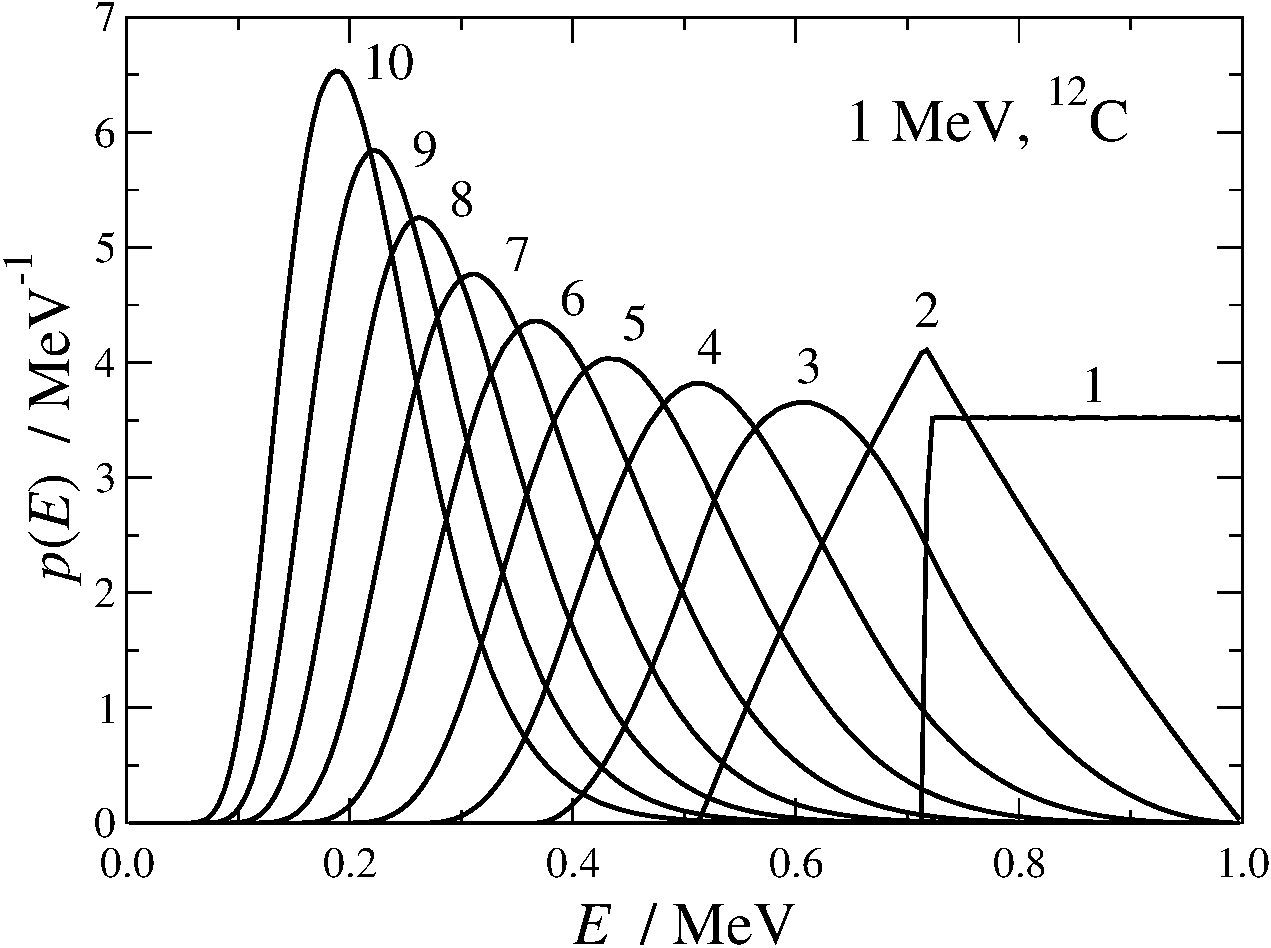
\includegraphics[width=6.0cm]{fig1.pdf}
\caption{A sample figure made smaller by changing the width parameter.}
\label{fig:small_sample}
\end{figure}



\vspace*{0.5cm}
\noindent
. . . . . . . . . . . . . . . . . . . . . . . . . . . . . . . . . . . . . . . .
. . . . . . . . . . . . . . . . . . . . . . . . . . . . . . . . . . . . . . . .
. . . . . . . . . . . . . . . . . . . . . . . . . . . . . . . . . . . . . . . .
. . . . . . . . . . . . . . . . . . . . . . . . . . . . . . . . . . . . . . . .
. . . . . . . . . . . . . . . . . . . . . . . . . . . . . . . . . . . . . . . .
. . . . . . . . . . . . . . . . . . . . . . . . . . . . . . . . . . . . . . . .
. . . . . . . . . . . . . . . . . . . . . . . . . . . . . . . . . . . . . . . .
. . . . . . . . . . . . . . . . . . . . . . . . . . . . . . . . . . . . . . . .
. . . . . . . . . . . . . . . . . . . . . . . . . . . . . . . . . . . . . . . .
. . . . . . . . . . . . . . . . . . . . . . . . . . . . . . . . . . . . . . . .
. . . . . . . . . . . . . . . . . . . . . . . . . . . . . . . . . . . . . . . .
. . . . . . . . . . . . . . . . . . . . . . . . . . . . . . . . . . . . . . . .
. . . . . . . . . . . . . . . . . . . . . . . . . . . . . . . . . . . . . . . .
. . . . . . . . . . . . . . . . . . . . . . . . . . . . . . . . . . . . . . . .
. . . . . . . . . . . . . . . . . . . . . . . . . . . . . . . . . . . . . . . .
. . . . . . . . . . . . . . . . . . . . . . . . . . . . . . . . . . . . . . . .
. . . . . . . . . . . . . . . . . . . . . . . . . . . . . . . . . . . . . . . .
. . . . . . . . . . . . . . . . . . . . . . . . . . . . . . . . . . . . . . . .
. . . . . . . . . . . . . . . . . . . . . . . . . . . . . . . . . . . . . . . .
. . . . . . . . . . . . . . . . . . . . . . . . . . . . . . . . . . . . . . . .
. . . . . . . . . . . . . . . . . . . . . . . . . . . . . . . . . . . . . . . .
. . . . . . . . . . . . . . . . . . . . . . . . . . . . . . . . . . . . . . . .
. . . . . . . . . . . . . . . . . . . . . . . . . . . . . . . . . . . . . . . .
. . . . . . . . . . . . . . . . . . . . . . . . . . . . . . . . . . . . . . . .
. . . . . . . . . . . . . . . . . . . . . . . . . . . . . . . . . . . . . . . .
. . . . . . . . . . . . . . . . . . . . . . . . . . . . . . . . . . . . . . . .
. . . . . . . . . . . . . . . . . . . . . . . . . . . . . . . . . . . . . . . .
. . . . . . . . . . . . . . . . . . . . . . . . . . . . . . . . . . . . . . . .
. . . . . . . . . . . . . . . . . . . . . . . . . . . . . . . . . . . . . . . .
. . . . . . . . . . . . . . . . . . . . . . . . . . . . . . . . . . . . . . . .
. . . . . . . . . . . . . . . . . . . . . . . . . . . . . . . . . . . . . . . .
. . . . . . . . . . . . . . . . . . . . . . . . . . . . . . . . . . . . . . . .
. . . . . . . . . . . . . . . . . . . . . . . . . . . . . . . . . . . . . . . .
. . . . . . . . . . . . . . . . . . . . . . . . . . . . . . . . . . . . . . . .
. . . . . . . . . . . . . . . . . . . . . . . . . . . . . . . . . . . . . . . .
. . . . . . . . . . . . . . . . . . . . . . . . . . . . . . . . . . . . . . . .
. . . . . . . . . . . . . . . . . . . . . . . . . . . . . . . . . . . . . . . .
. . . . . . . . . . . . . . . . . . . . . . . . . . . . . . . . . . . . . . . .
. . . . . . . . . . . . . . . . . . . . . . . . . . . . . . . . . . . . . . . .
. . . . . . . . . . . . . . . . . . . . . . . . . . . . . . . . . . . . . . . .

\subsection{Subsection 2}

. . . . . . . . . . . . . . . . . . . . . . . . . . . . . . . . . . . . . . . .
. . . . . . . . . . . . . . . . . . . . . . . . . . . . . . . . . . . . . . . .
. . . . . . . . . . . . . . . . . . . . . . . . . . . . . . . . . . . . . . . .
. . . . . . . . . . . . . . . . . . . . . . . . . . . . . . . . . . . . . . . .
. . . . . . . . . . . . . . . . . . . . . . . . . . . . . . . . . . . . . . . .
. . . . . . . . . . . . . . . . . . . . . . . . . . . . . . . . . . . . . . . .
. . . . . . . . . . . . . . . . . . . . . . . . . . . . . . . . . . . . . . . .
. . . . . . . . . . . . . . . . . . . . . . . . . . . . . . . . . . . . . . . .
. . . . . . . . . . . . . . . . . . . . . . . . . . . . . . . . . . . . . . . .
. . . . . . . . . . . . . . . . . . . . . . . . . . . . . . . . . . . . . . . .
. . . . . . . . . . . . . . . . . . . . . . . . . . . . . . . . . . . . . . . .
. . . . . . . . . . . . . . . . . . . . . . . . . . . . . . . . . . . . . . . .
. . . . . . . . . . . . . . . . . . . . . . . . . . . . . . . . . . . . . . . .
. . . . . . . . . . . . . . . . . . . . . . . . . . . . . . . . . . . . . . . .
. . . . . . . . . . . . . . . . . . . . . . . . . . . . . . . . . . . . . . . .
\section{Conclusions}
\begin{itemize}

\item
. . . . . . . . . . . . . . . . . . . . . . . . . . . . . . . . . . . . . . . .
. . . . . . . . . . . . . . . . . . . . . . . . . . . . . . . . . . . . . . . .
. . . . . . . . . . . . . . . . . . . . . . . . . . . . . . . . . . . . . . . .
. . . . . . . . . . . . . . . . . . . . . . . . . . . . . . . . . . . . . . . .
. . . . . . . . . . . . . . . . . . . . . . . . . . . . . . . . . . . . . . . .
. . . . . . . . . . . . . . . . . . . . . . . . . . . . . . . . . . . . . . . .
. . . . . . . . . . . . . . . . . . . . . . . . . . . . . . . . . . . . . . . .

\item
. . . . . . . . . . . . . . . . . . . . . . . . . . . . . . . . . . . . . . . .
. . . . . . . . . . . . . . . . . . . . . . . . . . . . . . . . . . . . . . . .
. . . . . . . . . . . . . . . . . . . . . . . . . . . . . . . . . . . . . . . .
. . . . . . . . . . . . . . . . . . . . . . . . . . . . . . . . . . . . . . . .
. . . . . . . . . . . . . . . . . . . . . . . . . . . . . . . . . . . . . . . .
. . . . . . . . . . . . . . . . . . . . . . . . . . . . . . . . . . . . . . . .
. . . . . . . . . . . . . . . . . . . . . . . . . . . . . . . . . . . . . . . .
\end{itemize}



\vspace*{0.5cm}
\begin{acknowledgments}
Be sure to thank your advisor,
your colleagues, and granting agencies (e.g. parents, etc...) as well.
\end{acknowledgments}

\begin{thebibliography}{99}

\bibitem{latex}Helmut Kopka and Patrick W. Daly, \textsl{A Guide to
\LaTeX: Document Preparation for Beginners and Advanced Users}, 3rd. ed. (Addison-Wesley, Reading, MA, 1999).

\bibitem{footnotes} It is necessary to process a file twice to
get the counters correct.

\bibitem{jackson} J.D. Jackson, {\it Classical Electrodynamics}, (John-Wiley
\& Sons, New York 1975, 2nd. ed.).


\bibitem{wmap} Hinshaw, G. et al. (WMAP Collaboration).
"Five-Year Wilkinson Microwave Anisotropy Probe Observations:
Data Processing, Sky Maps, and Basic Results".
The Astrophysical Journal Supplement {\bf 180}: 225–245 (2009).

\bibitem{weinberg} Weinberg, S.. "High-Energy Behavior in Quantum
Field Theory". Phys. Rev. {\bf 118}: 838–849 (1960).


\end{thebibliography}

\clearpage


\title{Preparaci\'o del manuscript del TFG amb \LaTeX}

\begin{abstract}
{\bf Resum:} En aquesta sisena p\`agina cal incloure la informaci\'o b\`asica en la llengua oficial de la UB, que \'es el catal\`a. Concretament, \'es necessari el t\'itol, el resum del contingut i les paraules clau. Es convida als estudiants a afegir-hi (opcional, per\`o sempre dins de la sisena p\`agina) un resum visual (Graphical Abstract), \'es a dir un resum \'unic, conc\'is i visual de les principals conclusions del treball. Podria ser la figura del resultat final o, millor encara, una figura especialment dissenyada per a aquest prop\`osit, que mostri d'un sol cop d'ull el contingut del TFG.
\keywordcat{Fins a 6 paraules que relacionin el treball amb conceptes estudiats al grau de F\'isica.}
\ods{Aquest TFG est\`a relacionat amb els Objectius de Desenvolupament Sostenible (SDGs)}
\end{abstract}

\maketitle
\thispagestyle{fancy}


\onecolumngrid
\vspace{-1.5cm}
\section*{Objectius de Desenvolupament Sostenible (ODSs o SDGs)}
\vspace{-0.5cm}
\begin{table}[h]
\begin{center}
\begin{tabular}{|l|c|l|c|}
\hline
1. Fi de la es desigualtats & & 10. Reducci\'o de les desigualtats &\\ \hline
2. Fam zero	               &  &	11. Ciutats i comunitats sostenibles	& \\  \hline
3. Salut i benestar	      &  &	12. Consum i producci\'o responsables& \\  \hline	
4. Educaci\'o de qualitat   & X &	13. Acci\'o clim\`atica	& X \\  \hline
5. Igualtat de g\`enere	      &  &	14. Vida submarina	& \\  \hline
6. Aigua neta i sanejament &  &	15. Vida terrestre	& \\  \hline
7. Energia neta i sostenible & X &	16. Pau, just\'icia i institucions s\`olides	& \\  \hline
8. Treball digne i creixement econ\`omic &  & 17. Alian\c{c}a pels objectius	& \\  \hline
9. Ind\'ustria, innovaci\'o, infraestructures &  &  & \\
\hline
\end{tabular}
\end{center}
\label{default}
\end{table}
\vspace{-0.5cm}
Es pot incloure un breu par\`agraf subratllant la relaci\'o entre aquest TFG i els ODSs i les seves fites espec\'ifiques (disponibles a https://www.diba.cat/web/ods/coneix-els-ods i a https://sdgs.un.org/goals). Per exemple: ``El contingut d'aquest TFG, part d'un grau universitari de F\'isica, es relaciona amb l'ODS 4, i en particular amb la fita 4.4, ja que contribueix a l'educaci\'o a nivell universitari. Tamb\'e es pot relacionar amb l'ODS 7, fita 7.2, perqu\`e s'estudia energies renovables, i amb l'ODS 13, fita 13.4, perqu\`e promou l'educaci\'o, mitigaci\'o, adaptaci\'o i reducci\'o de l'impacte del canvi clim\`atic.''
\vspace{-0.5cm}
\section*{GRAPHICAL ABSTRACT (OPTIONAL)}
\vspace{-0.5cm}
\begin{figure}[h]
\centering
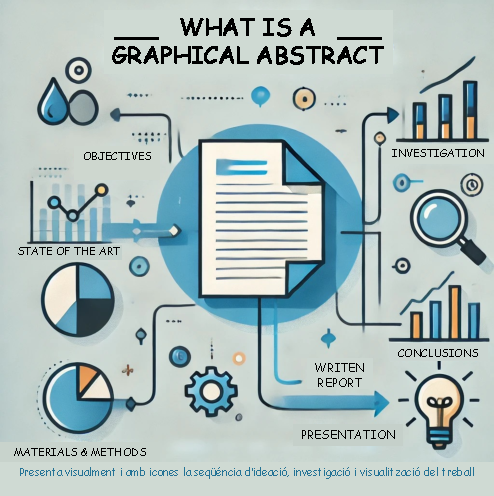
\includegraphics[width=8.5cm]{VisualAbstract.pdf}
\end{figure}




\clearpage
\twocolumngrid
\appendix
\section{SUPPLEMENTARY MATERIAL (OPTIONAL)}

Here, you may add supplementary materials that are relevant but not essential if needed. These can include data from databases, programming code, figures, tables, equations, etc., in any format. Note that these materials will not be evaluated by the jury and may not even be viewed. For example, the following equation,
\begin{equation} 
\vec{F}=m \vec{a} 
\end{equation}
is important in physics.




\end{document}
